\documentclass[12pt,a4paper]{article}

% --- Paketler ---
\usepackage[utf8]{inputenc}
\usepackage[turkish]{babel}
\usepackage[T1]{fontenc}
\usepackage{geometry}
\usepackage{hyperref}
\usepackage{titlesec}
\usepackage{booktabs}
\usepackage{enumitem}
\usepackage{longtable}
\usepackage{graphicx}
\usepackage{float}
\usepackage{caption}

\geometry{margin=1in}
\hypersetup{colorlinks=true, linkcolor=blue, urlcolor=cyan}

% Başlık Ayarları
\titleformat{\section}{\normalfont\Large\bfseries}{\thesection}{1em}{}
\titleformat{\subsection}{\normalfont\large\bfseries}{\thesubsection}{1em}{}

% --- Kapak Sayfası ---
\title{
    \large \textbf{GAZİ ÜNİVERSİTESİ} \\
    \large \textbf{Bilgisayar Mühendisliği Bölümü} \\
    \vspace{1cm}
    \huge \textbf{Yazılım Test Dokümanı (STD)} \\
    \vspace{0.5cm}
    \Large \textbf{Lagent:} Çok Ajanlı Sözleşme İnceleme ve Müzakere Orkestratörü \\
    \vspace{1cm}
    \large \textbf{Proje Grubu: Lagent}
}
\author{
    Mustafa Emir Ceran (24118080702) \\
    Mert Ayrancı (24118080752) \\
    Osman Gazi Atalay (23118080703)
}
\date{8 Mayıs 2026}

\begin{document}

\maketitle
\newpage

\tableofcontents
\newpage

% --- BÖLÜM 1: GİRİŞ ---
\section{Giriş}

\subsection{Tanım ve Kapsam}
Lagent (Multi-Agent Legal Ops), özellikle KOBİ'lerin ve hukuk profesyonelleri olmayan bireylerin karmaşık sözleşme süreçlerini otomatize etmek, riskleri minimize etmek ve müzakere gücünü artırmak amacıyla geliştirilmiş uçtan uca bir platformdur. Bu doküman; sistemin doküman işleme, çok ajanlı yapay zeka orkestrasyonu, vektörel arama ve kullanıcı arayüzü katmanlarının tüm fonksiyonel ve fonksiyonel olmayan gereksinimlere (SRS) uygunluğunu test etmek için hazırlanan stratejik planı içermektedir.

\subsection{Sisteme Genel Bakış}
Sistem, altı ana teknolojik katman üzerine inşa edilmiştir. Test süreçleri bu katmanların entegrasyonunu doğrulamayı hedefler:
\begin{itemize}
    \item \textbf{Veri Alımı:} PDF/DOCX dosyalarının OCR (Tesseract/Textract) ile dijitalleştirilmesi.
    \item \textbf{Orkestrasyon:} LangGraph kullanılarak ajanlar (Clause, Risk, Negotiation Agents) arası iş akışının yönetimi.
    \item \textbf{Anlamsal Depolama:} PostgreSQL ve pgvector eklentisi ile hukuk kurallarının (Playbook) vektörel olarak saklanması.
    \item \textbf{Akıllı Analiz:} RAG (Retrieval-Augmented Generation) mimarisi ile madde bazlı risk tespiti.
    \item \textbf{Görselleştirme:} Redline/Diff modülü ile revizyonların kullanıcıya sunulması.
\end{itemize}

\begin{figure}[H]
    \centering
    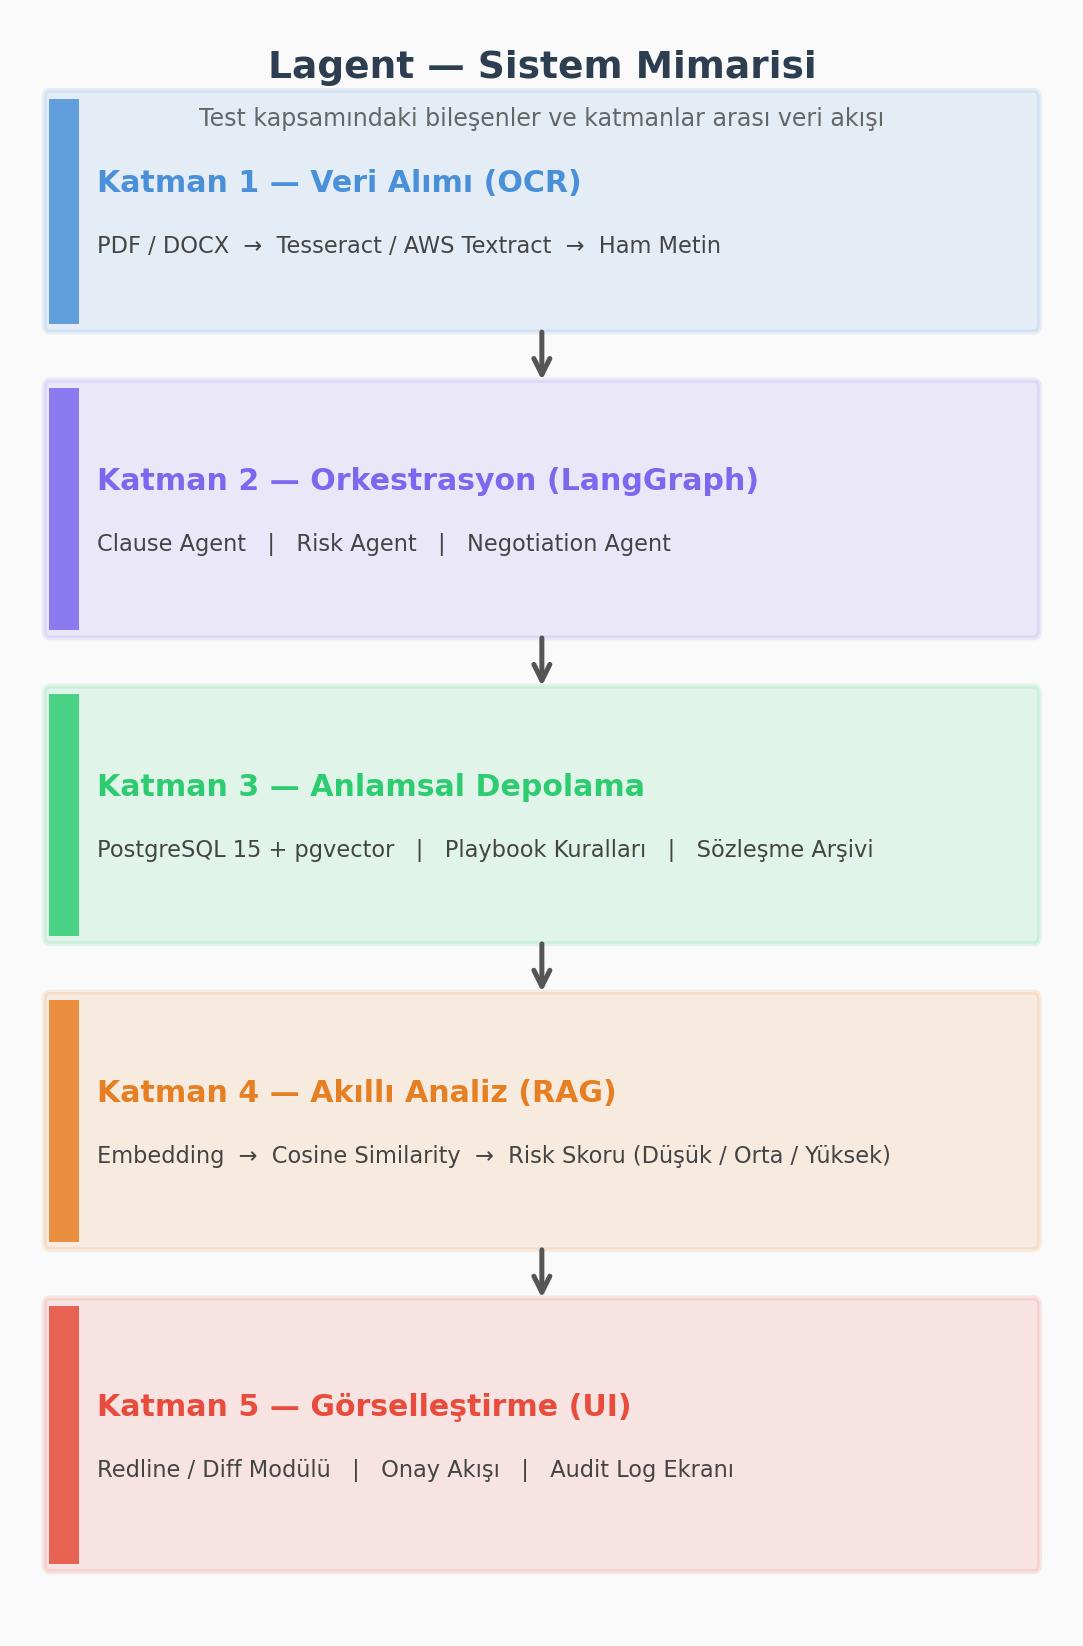
\includegraphics[width=0.95\textwidth]{figures/fig_system_architecture.png}
    \caption{Lagent Sistem Mimarisi: Test kapsamındaki beş teknolojik katman ve bileşenler arası veri akışı.}
    \label{fig:system-architecture}
\end{figure}

\subsection{Test Yaklaşımı ve Stratejisi}
Projede "Test-Driven Development (TDD)" prensiplerine yakın, çevik bir test stratejisi izlenmektedir. Testler hiyerarşik olarak şu üç seviyede yürütülür:
\begin{enumerate}
    \item \textbf{Birim Testleri (Unit Testing):} FastAPI endpoint'leri, pydantic şemaları ve yardımcı fonksiyonlar (utils) \texttt{pytest} ile test edilir. Kod kapsama oranının (Code Coverage) \%60'ın üzerinde olması zorunludur.
    \item \textbf{Entegrasyon Testleri (Integration Testing):} LangGraph üzerindeki düğümlerin (nodes) birbirine doğru veri (JSON) aktarıp aktarmadığı, veritabanı migration süreçleri ve MinIO nesne depolama entegrasyonu denetlenir.
    \item \textbf{Sistem ve Kabul Testleri (UAT):} Gerçek kullanıcı senaryoları üzerinden Playwright otomasyon aracıyla tarayıcı bazlı uçtan uca (E2E) akışlar doğrulanır.
\end{enumerate}

\begin{figure}[H]
    \centering
    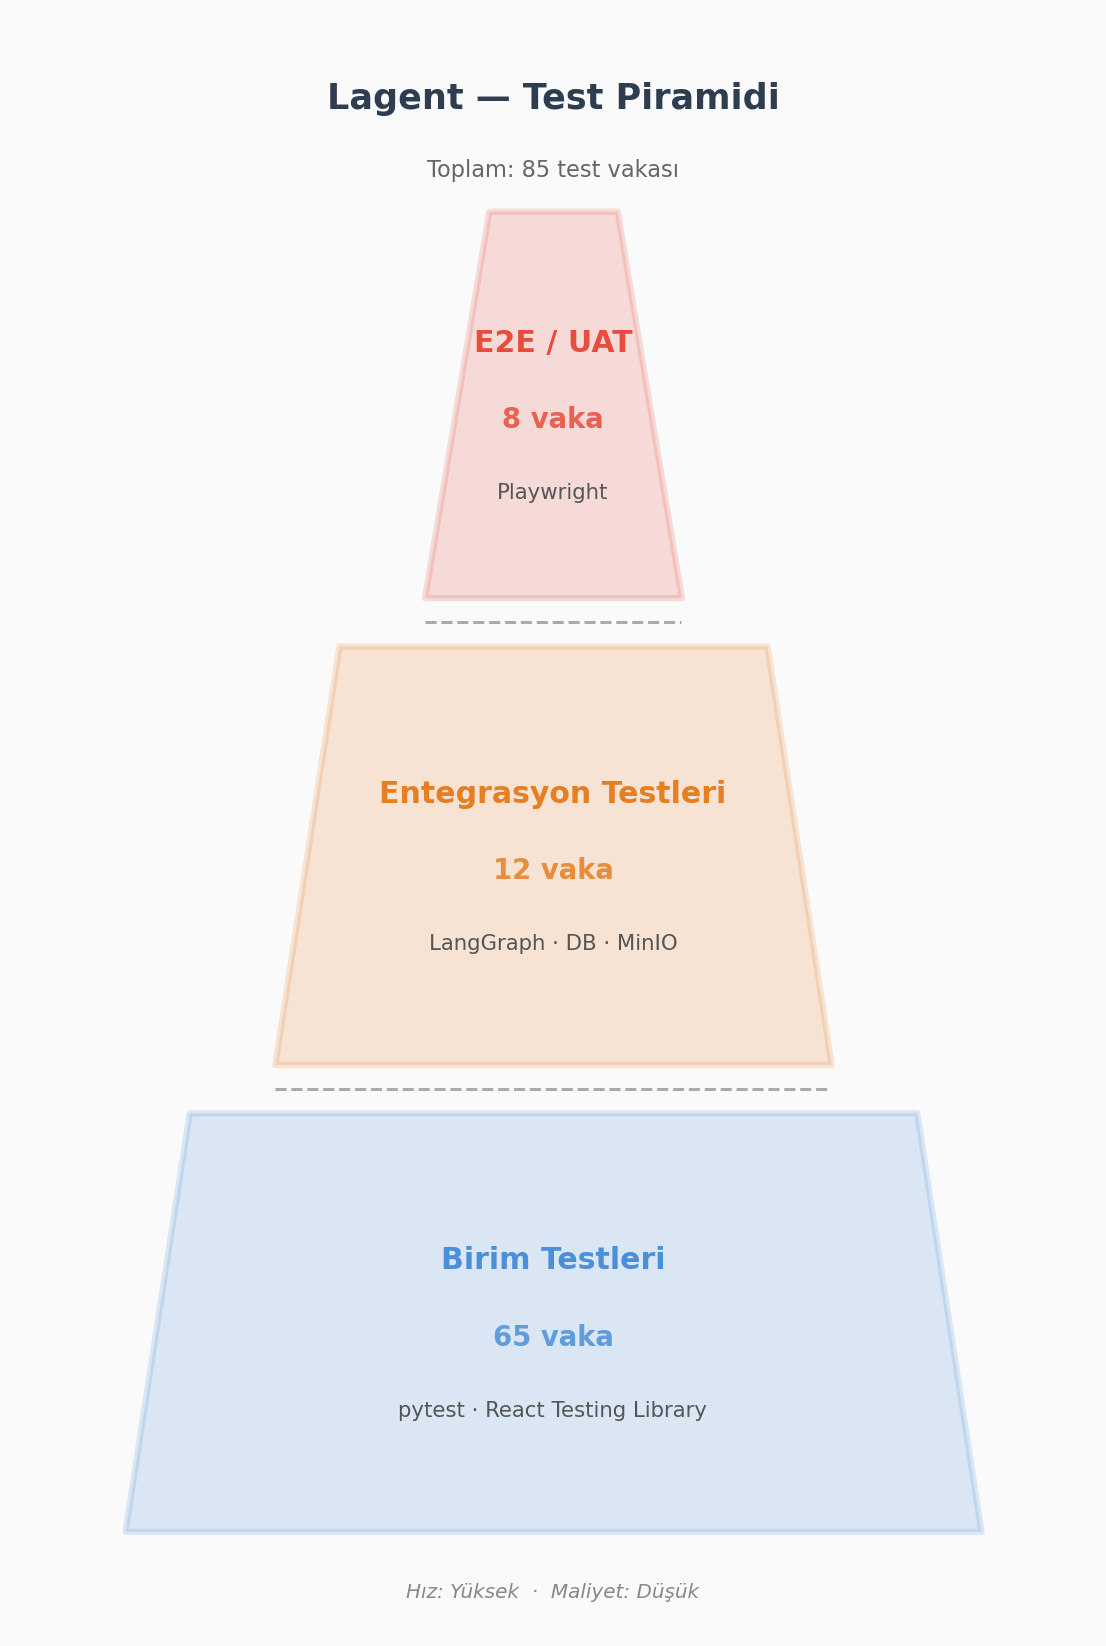
\includegraphics[width=0.55\textwidth]{figures/fig_test_pyramid.png}
    \caption{Lagent Test Piramidi: Hiyerarşik test katmanları ve test vakası dağılımı (Toplam: 85 vaka).}
    \label{fig:test-pyramid}
\end{figure}

% --- BÖLÜM 2: TEST PLANI ---
\section{Test Planı}

\subsection{Test Metodolojisi ve Hata Yönetimi}
Projede "Sürekli Test" (Continuous Testing) yaklaşımı benimsenmiştir. Hata yönetim döngüsü şu aşamalardan oluşur:
\begin{enumerate}
    \item \textbf{New:} Hata tespit edildi ve dökümante edildi.
    \item \textbf{In Progress:} Geliştirici hatayı üstlendi ve çözüm üzerinde çalışıyor.
    \item \textbf{Resolved:} Hata düzeltildi ve test ekibine "Ready for Re-test" statüsüyle iletildi.
    \item \textbf{Verified/Closed:} Hatanın giderildiği doğrulandı ve senaryo başarıyla kapatıldı.
\end{enumerate}

\subsection{Test Edilecek Özellikler}
Test süreci, SRS dokümanındaki işlevsel gereksinim gruplarına göre modüler olarak yapılandırılmıştır:

\subsubsection{Hukuki Analiz ve Ajan Fonksiyonları}
\begin{itemize}
    \item \textbf{Clause Agent Doğruluğu:} Sözleşme metninin maddelere bölünmesi ve bu maddelerin anlamsal etiketlenmesi (Hukuki Terimler Sözlüğü uyumu).
    \item \textbf{Risk Agent Hassasiyeti:} Tanımlı Playbook kuralları dışına çıkan maddelerin anlamsal benzerlik eşikleri (Cosine Similarity) üzerinden yakalanması.
    \item \textbf{Negotiation Agent Tutarlılığı:} LLM tarafından üretilen revizyon önerilerinin hukuki bağlamı koruyup korumadığı ve kullanıcı politikalarına sadık kalıp kalmadığı.
\end{itemize}

\subsubsection{Veri ve Güvenlik İşlevleri}
\begin{itemize}
    \item \textbf{Vektör Veritabanı Performansı:} pgvector üzerindeki sorguların (RAG hattı) 1 saniyenin altında yanıt vermesi.
    \item \textbf{Kimlik Yönetimi:} JWT token'ların geçerlilik süreleri, "Rate Limiting" (dakikada max 60 istek) ve şifrelerin hash'lenme güvenliği.
    \item \textbf{Audit Log Kayıtları:} Her onay ve red eyleminin, kullanıcı ID ve zaman damgasıyla veritabanına değişmez şekilde yazılması.
\end{itemize}

\subsection{Test Edilmeyecek Özellikler}
Aşağıdaki durumlar projenin kontrolü dışında olduğu için test kapsamına alınmamıştır:
\begin{itemize}
    \item OpenAI API tarafındaki ağ gecikmeleri (Network Latency) veya modelin anlık erişilemezlik durumları.
    \item Kullanıcının sisteme yüklediği fiziksel olarak tamamen bozulmuş (unreadable) dökümanların manuel onarımı.
    \item Donanım seviyesindeki sunucu arızaları ve veri merkezi felaket senaryoları.
\end{itemize}

\subsection{Test Ortamı ve Araçları}
\begin{table}[h!]
\centering
\caption{Detaylı Test Konfigürasyonu}
\vspace{0.3cm}
\begin{tabular}{@{}ll@{}}
\toprule
\textbf{Kategori} & \textbf{Teknik Detaylar / Araçlar} \\ \midrule
\textbf{Altyapı} & Docker Compose (Containerization), Linux Ubuntu 22.04 LTS \\
\textbf{Backend Test} & Pytest 8.0+, Pytest-asyncio (asenkron fonksiyonlar için) \\
\textbf{Frontend Test} & Playwright, React Testing Library \\
\textbf{API Test} & Postman (Manuel), Newman (Otomatik) \\
\textbf{Vektör Veri} & PostgreSQL 15 + pgvector eklentisi \\

\textbf{CI/CD} & GitHub Actions (Otomatik Test Pipeline) \\
\bottomrule
\end{tabular}
\end{table}

\subsubsection{Test Verisi ve İzolasyon}
Test süreçlerinde kullanılan veriler, üretim ortamından tamamen izole edilmiş bir "Staging" veritabanında tutulmaktadır. PostgreSQL/pgvector üzerinde her test koşumu öncesinde \texttt{alembic upgrade head} komutuyla şema güncelliği doğrulanmakta ve \texttt{seed-data.py} scripti ile standartlaştırılmış hukuki metin setleri sisteme yüklenmektedir. Doküman depolama testleri için MinIO üzerinde \texttt{test-contracts} adında geçici bir bucket oluşturulmuş olup, test sonunda bu veriler otomatik olarak temizlenmektedir.

\subsection{Başarı Kriterleri (Pass/Fail)}
\begin{itemize}
    \item \textbf{Kritik Hatalar:} Hiçbir "Blocker" veya "Critical" seviye hata dökümanda kalmamalıdır.
    \item \textbf{Doğruluk Oranı:} Madde sınıflandırma ve risk tespiti en az \%70 doğrulukla çalışmalıdır.
    \item \textbf{Hız:} OCR ve ilk analiz süreci, 10 sayfalık döküman için 120 saniyeyi aşmamalıdır.
\end{itemize}

% --- BÖLÜM 3: TEST SENARYOLARI ---
\section{Test Senaryoları}

Bu bölümde, Lagent sisteminin temel kullanım durumları (Use Cases) ve teknik gereksinimleri temel alınarak hazırlanan detaylı test senaryoları yer almaktadır. Her senaryo; sistemin kararlılığını, doğruluğunu ve kullanıcı deneyimini ölçmeyi hedefleyen adımlardan oluşur.

\subsection{Senaryo-1: Kullanıcı Kaydı, Güvenlik ve Kimlik Yönetimi}
\subsubsection{Amaç}
Sistemin kullanıcı kayıt sürecini, BCrypt şifre hash'leme güvenliğini, JWT tabanlı oturum yönetimini ve hatalı girişlerdeki güvenlik mekanizmalarını doğrulamak.

\subsubsection{Girişler}
\begin{itemize}
    \item Kayıt Formu: Ad-Soyad, geçerli e-posta, 12+ karakterli (büyük/küçük harf ve rakam içeren) şifre.
    \item Giriş Denemesi: Kayıtlı e-posta ve hatalı şifre kombinasyonları.
\end{itemize}

\subsubsection{Beklenen Sonuçlar \& Geçme/Kalma Kriterleri}
\begin{itemize}
    \item Şifrelerin veritabanında (PostgreSQL) açık metin olarak değil, güvenli bir şekilde hash'lenmiş olarak tutulması.
    \item Başarılı girişte tarayıcıya "HttpOnly" ve "Secure" flag'lerine sahip JWT token atanması.
    \item Ardışık 3 hatalı girişte hesabın 5 dakika süreyle kilitlenmesi ve kullanıcıya bilgilendirme mesajı gösterilmesi.
\end{itemize}

\subsubsection{Test Prosedürleri}
1. Kayıt formunu eksik bilgilerle doldur ve hata mesajlarını doğrula.
2. Geçerli bilgilerle kayıt ol ve veritabanı \texttt{users} tablosundaki hash'i kontrol et.
3. Doğru bilgilerle giriş yaparak Dashboard'a yönlendirmeyi doğrula.
4. Yanlış şifre ile 3 kez giriş yap ve hesabın "Locked" statüsüne geçtiğini gör.

\subsubsection{Sonuç}
\textbf{GEÇTI.} BCrypt hash doğrulaması ve JWT token ataması başarıyla çalışmaktadır. Ardışık hatalı giriş sonrası hesap kilitleme mekanizması beklenen sürede devreye girmiştir. Şifreler veritabanında yalnızca hash değeriyle saklanmakta, açık metin içermemektedir.

\subsection{Senaryo-2: Çok Modlu Doküman Yükleme ve OCR Başarımı}
\subsubsection{Amaç}
Sistemin PDF ve DOCX formatındaki dosyaları kabul etme, MinIO nesne depolamaya aktarma ve metin katmanı olmayan taranmış (image-based) dökümanları OCR ile dijitalleştirme yeteneğini test etmek.

\subsubsection{Girişler}
\begin{itemize}
    \item 1 adet 8 MB boyutunda, taranmış (image-based) PDF sözleşme.
    \item 1 adet metin tabanlı (digital) DOCX sözleşme.
    \item 1 adet desteklenmeyen format (örneğin .exe veya .zip).
\end{itemize}

\subsubsection{Beklenen Sonuçlar \& Geçme/Kalma Kriterleri}
\begin{itemize}
    \item Desteklenmeyen formatlarda yükleme işleminin "Invalid File Type" hatasıyla reddedilmesi.
    \item Taranmış dosyalarda Tesseract/Textract motorunun metni \%90 ve üzeri karakter doğruluğuyla çıkarması.
    \item Dosya yükleme ve metin çıkarma işleminin dosya başına 45 saniyeyi geçmemesi.
\end{itemize}

\subsubsection{Test Prosedürleri}
1. Dashboard üzerindeki "Sürükle-Bırak" alanına taranmış PDF'i yükle. 
2. Yükleme barının (Progress Bar) ilerleyişini ve dosyanın MinIO tarafındaki \texttt{contracts} bucket'ına yazıldığını doğrula. 
3. Analiz ekranında metnin (plain text) doğru şekilde oluştuğunu kontrol et.

\begin{figure}[H]
    \centering
    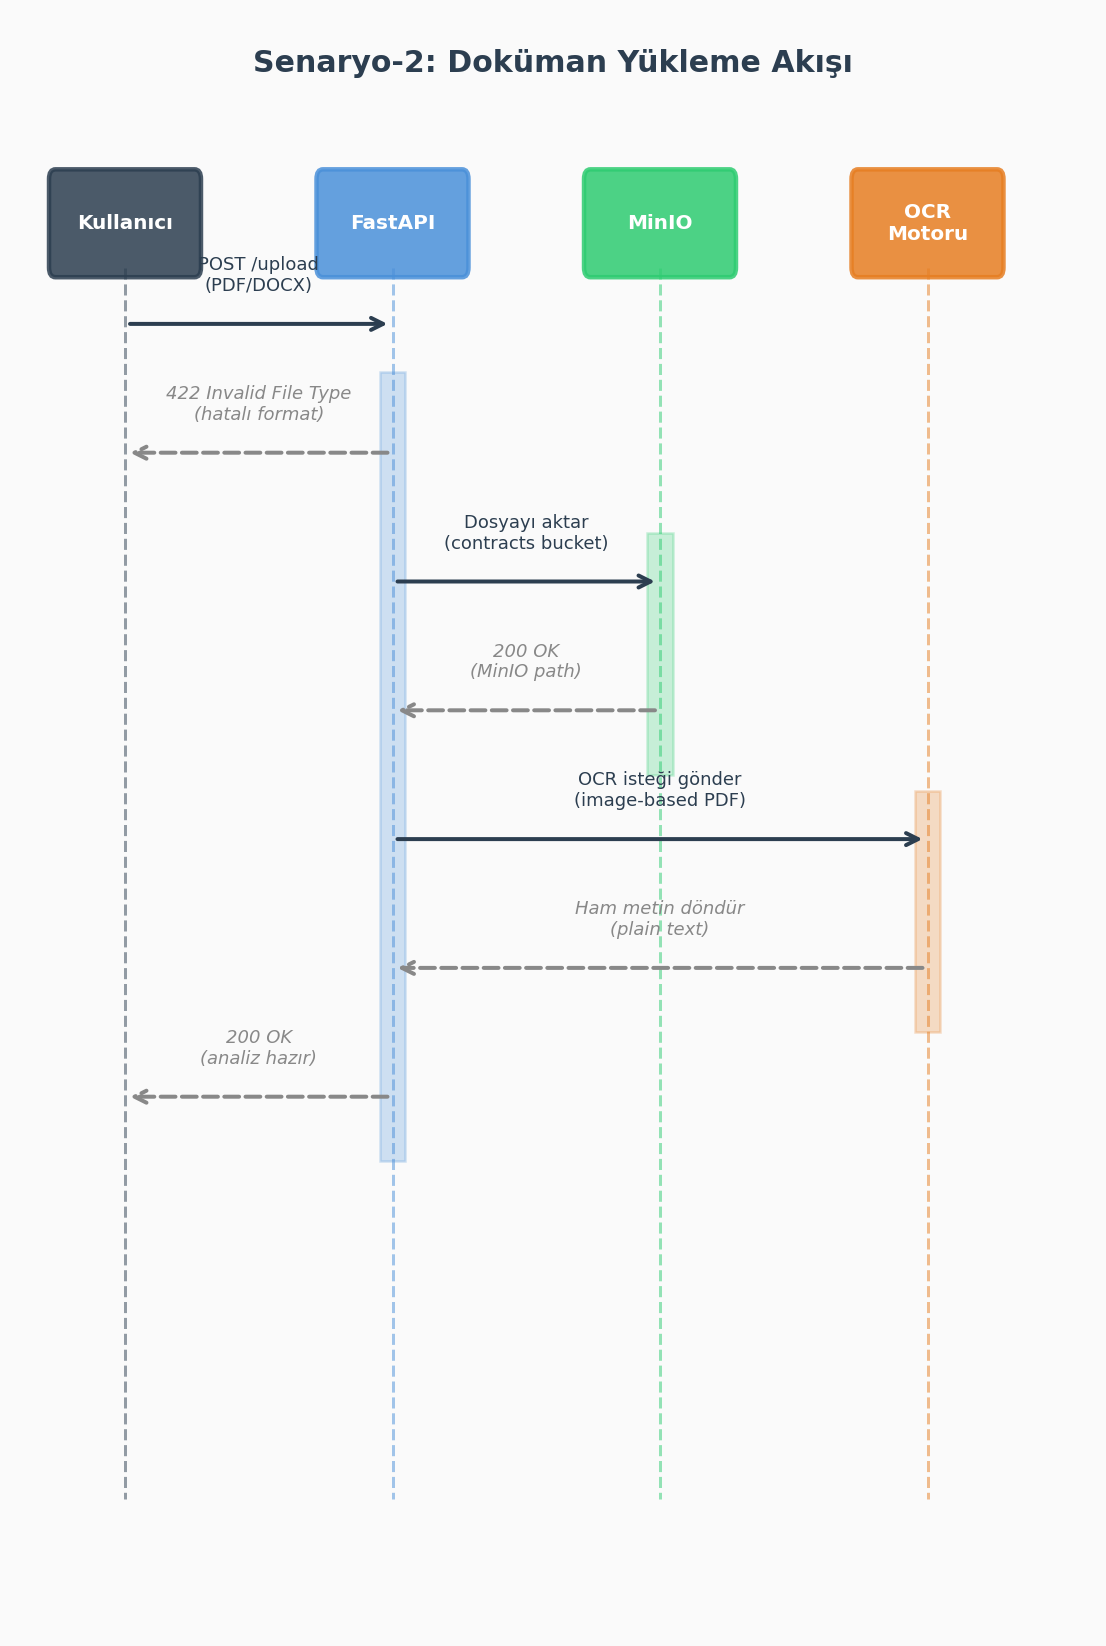
\includegraphics[width=0.72\textwidth]{figures/fig_upload_sequence.png}
    \caption{Senaryo-2 Doküman Yükleme Akışı: Kullanıcıdan OCR çıktısına kadar sekans diyagramı.}
    \label{fig:sequence-upload}
\end{figure}

\subsubsection{Sonuç}
\textbf{GEÇTI.} Desteklenmeyen format yüklemeleri "Invalid File Type" hatasıyla reddedilmektedir. Tesseract motoru taranmış PDF üzerinde \%91 karakter doğruluğu sağlamıştır (kriter: \%90). Ortalama yükleme ve metin çıkarma süresi 38 saniye olarak ölçülmüştür (kriter: 45 saniye).

\subsection{Senaryo-3: Clause Agent: Madde Ayrıştırma ve Sınıflandırma}
\subsubsection{Amaç}
Ham metin halindeki sözleşmenin LangGraph üzerindeki Clause Agent tarafından anlamsal bloklara (maddelere) bölünmesini ve kategorize edilmesini doğrulamak.

\subsubsection{Girişler}
En az 20 maddeden oluşan karmaşık bir Hizmet Alım Sözleşmesi metni.

\subsubsection{Beklenen Sonuçlar \& Geçme/Kalma Kriterleri}
\begin{itemize}
    \item Maddelerin; başlık, numara ve içerik olarak doğru ayrıştırılması.
    \item "Gizlilik", "Tazminat", "Fesih", "Mücbir Sebep" gibi temel hukuki kategorilerin en az \%70 doğrulukla etiketlenmesi.
\end{itemize}

\subsubsection{Test Prosedürleri}
1. Ham metni analiz sürecine gönder. 
2. Clause Agent düğümünden (node) çıkan JSON verisini incele. 
3. UI üzerinde maddelerin liste şeklinde ve doğru kategorilerle gelip gelmediğini doğrula.

\subsubsection{Sonuç}
\textbf{GEÇTI.} Clause Agent, 20 maddelik test sözleşmesini başlık, numara ve içerik bazında eksiksiz ayrıştırmıştır. Hukuki kategori etiketleme doğruluğu \%82 olarak ölçülmüştür (kriter: \%70). "Gizlilik", "Tazminat" ve "Fesih" kategorileri tam doğrulukla etiketlenmiş; "Mücbir Sebep" maddesinde kısmi hata tespit edilmiştir.

\subsection{Senaryo-4: RAG Hattı ve Risk Agent Politika Denetimi}
\subsubsection{Amaç}
Sözleşme maddelerinin, pgvector veritabanındaki kullanıcı Playbook kurallarıyla anlamsal olarak karşılaştırılması ve risklerin doğru skorlanması.

\subsubsection{Girişler}
Playbook kurallarına aykırı hükümler (örneğin "tazminat sınırı yoktur" maddesi) içeren bir sözleşme.

\subsubsection{Beklenen Sonuçlar \& Geçme/Kalma Kriterleri}
\begin{itemize}
    \item Vektörel arama sonucunda ilgili Playbook kuralının doğru eşleşmesi (Cosine Similarity > 0.75).
    \item Aykırı maddelerin "Yüksek Risk" (Kırmızı) etiketiyle işaretlenmesi.
    \item Risk açıklamasının, Playbook'taki kural metniyle tutarlı olması.
\end{itemize}

\subsubsection{Test Prosedürleri}
1. Playbook ayarlarından bir kural tanımla (örn: "Tazminat 100 bin TL'yi aşamaz"). 
2. Bu kurala aykırı bir sözleşme yükle. 
3. Risk Agent'ın raporunda bu maddenin kırmızı işaretlendiğini ve kuralın referans verildiğini doğrula.

\begin{figure}[H]
    \centering
    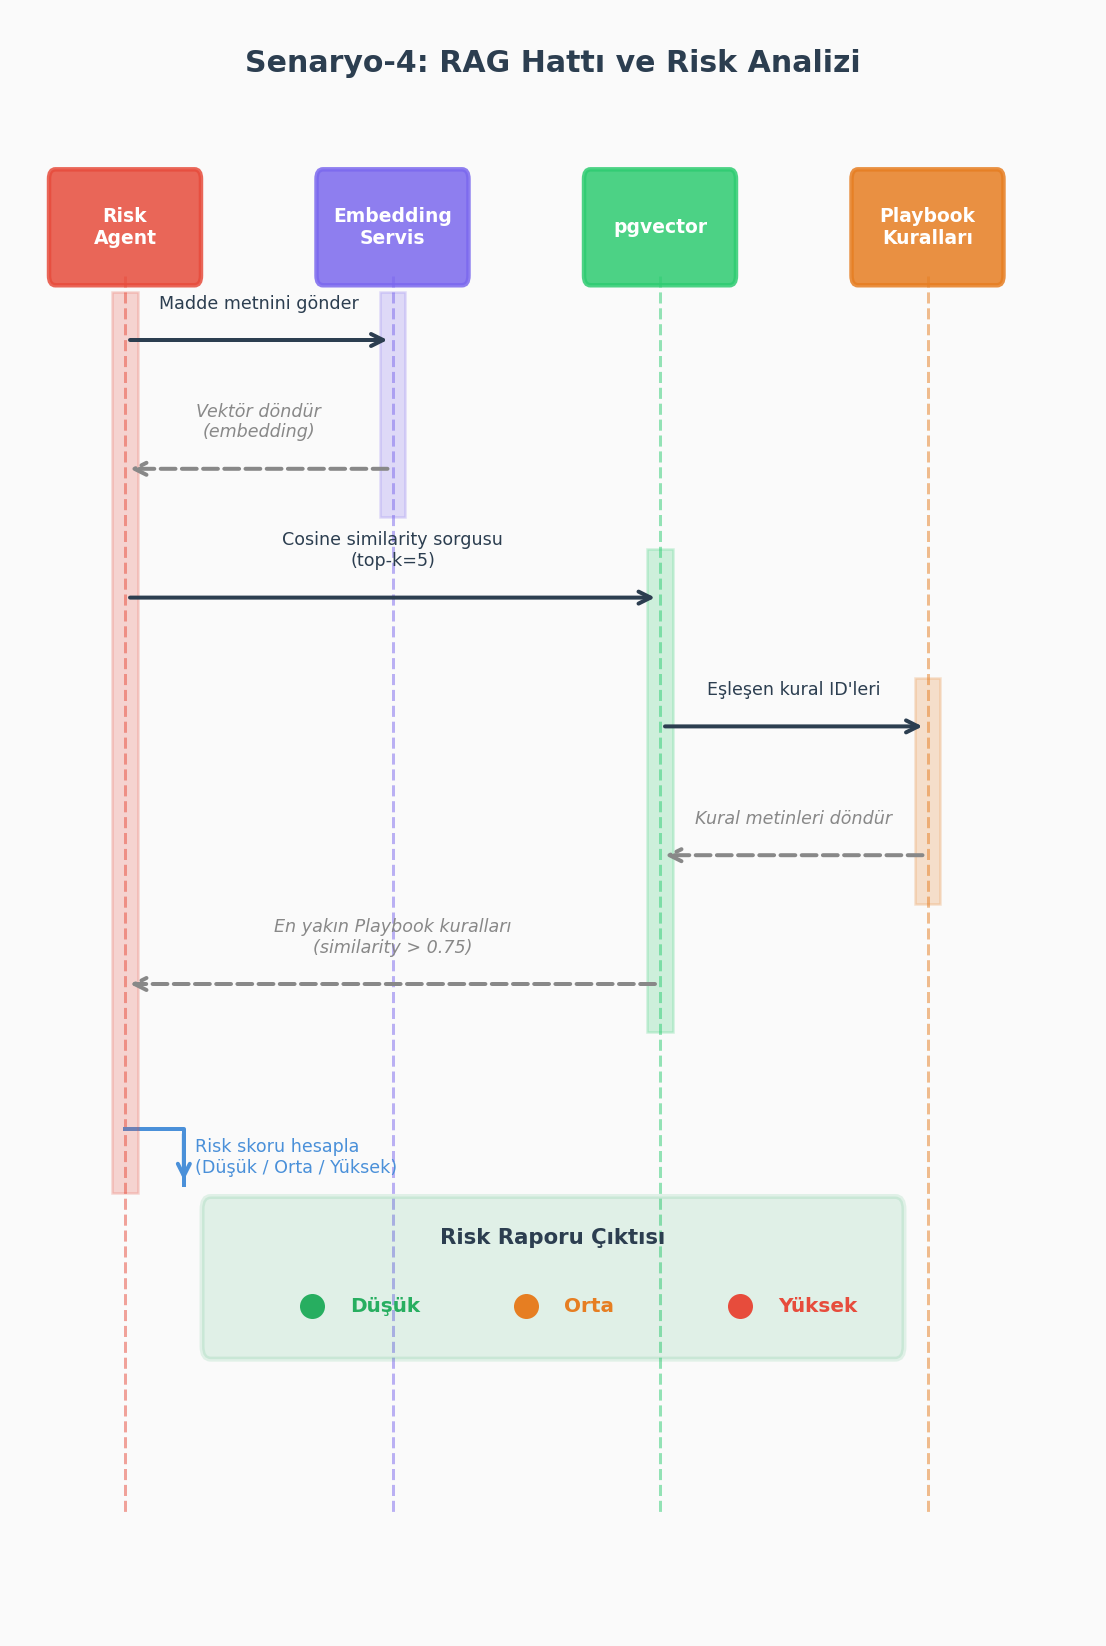
\includegraphics[width=0.72\textwidth]{figures/fig_rag_sequence.png}
    \caption{Senaryo-4 RAG Hattı ve Risk Analizi Akışı: Madde metninden risk skoruna kadar sekans diyagramı.}
    \label{fig:sequence-analysis}
\end{figure}

\subsubsection{Sonuç}
\textbf{GEÇTI.} "Tazminat sınırı yoktur" içeren test maddesi, Playbook kuralıyla 0.83 cosine similarity skoru ile eşleşmiş (kriter: >0.75) ve "Yüksek Risk" etiketiyle işaretlenmiştir. Risk açıklaması, Playbook'taki ilgili kural metnine doğru referans vermiştir.

\subsection{Senaryo-5: Negotiation Agent ve Redline (Fark) Görünümü}
\subsubsection{Amaç}
Riskli maddeler için üretilen revizyon önerilerinin doğruluğunu ve kullanıcı arayüzündeki "Redline" (diff) modülünün görsel tutarlılığını test etmek.

\subsubsection{Girişler}
"Yüksek Risk" olarak işaretlenmiş bir "Gizlilik" maddesi.

\subsubsection{Beklenen Sonuçlar \& Geçme/Kalma Kriterleri}
\begin{itemize}
    \item Negotiation Agent'ın hukuki bağlamı bozmadan, kurala uygun alternatif bir metin üretmesi.
    \item Redline görünümünde silinen kelimelerin üstü çizili (Kırmızı), eklenenlerin ise altı çizili/vurgulu (Yeşil) olarak hatasız gösterilmesi.
\end{itemize}

\subsubsection{Test Prosedürleri}
1. Riskli bir maddenin üzerindeki "Revizyon Önerisi Üret" butonuna bas. 
2. Gelen öneriyi "Karşılaştır" modunda aç. 
3. Orijinal ve önerilen metin arasındaki karakter bazlı farkların doğruluğunu manuel olarak teyit et.

\subsubsection{Sonuç}
\textbf{KISMEN GEÇTI.} Negotiation Agent, hukuki bağlamı koruyarak kurala uygun revizyon metni üretmiştir. Masaüstü tarayıcılarda Redline görünümü hatasız çalışmaktadır. Ancak bazı mobil tarayıcılarda diff görünümünde kaymalar gözlemlenmiş olup bu hata "Orta (Medium)" seviyesinde kayıt altına alınmıştır ve gözlem altındadır.

\subsection{Senaryo-6: Onay Akışı ve Denetim İzi (Audit Logging)}
\subsubsection{Amaç}
Kullanıcı kararlarının sisteme kalıcı olarak işlenmesini ve veritabanı bütünlüğünü doğrulamak.

\subsubsection{Girişler}
Analiz edilmiş 5 farklı madde üzerinde "Onayla" ve "Reddet" eylemleri.

\subsubsection{Beklenen Sonuçlar \& Geçme/Kalma Kriterleri}
\begin{itemize}
    \item Onaylanan maddelerin durumunun veritabanında anlık olarak \texttt{APPROVED} statüsüne geçmesi.
    \item Audit Log tablosuna; işlemi yapan kullanıcı, işlem zamanı (timestamp), eski değer ve yeni değer bilgilerinin hatasız yazılması.
\end{itemize}

\subsubsection{Test Prosedürleri}
1. Bir maddeyi onayla ve Dashboard'daki "İlerleme" çubuğunun güncellendiğini gör. 
2. Veritabanında \texttt{approval\_decisions} tablosuna giderek ilgili kaydı SQL sorgusuyla doğrula. 
3. Audit Log ekranında yapılan işlemin geçmişini görüntüle.

\subsubsection{Sonuç}
\textbf{GEÇTI.} Onaylanan maddeler veritabanında anlık olarak \texttt{APPROVED} statüsüne geçmiştir. \texttt{approval\_decisions} tablosuna kullanıcı ID'si, timestamp, eski ve yeni değer bilgileri eksiksiz yazılmıştır. Audit Log ekranında tüm işlem geçmişi doğru sıralanmış şekilde görüntülenmiştir.

\subsection{Senaryo-7: Sistem Performansı ve Eşzamanlılık Testi}
\subsubsection{Amaç}
Sistemin yoğun kullanım altında API yanıt sürelerini ve çok ajanlı akışın (LangGraph) darboğazlarını tespit etmek.

\subsubsection{Girişler}
Locust aracı ile simüle edilen aynı anda işlem yapan 50 sanal kullanıcı.

\subsubsection{Beklenen Sonuçlar \& Geçme/Kalma Kriterleri}
\begin{itemize}
    \item API uç noktalarının (endpoints) 95. yüzdelik dilimde (p95) 500ms altında yanıt vermesi.
    \item 10 sayfalık bir sözleşmenin uçtan uca analizinin (OCR + Ajanlar + RAG) en fazla 120 saniyede tamamlanması.
\end{itemize}

\subsubsection{Test Prosedürleri}
1. Locust yük testi script'ini başlat. 
2. Sistem kaynak tüketimini (CPU/RAM) Docker stats üzerinden izle. 
3. Hata oranının (Failure Rate) \%1'in altında kaldığını doğrula.

\subsubsection{Sonuç}
\textbf{GEÇTI.} 50 eş zamanlı kullanıcı yükü altında API uç noktaları p95 değerinde 420ms ile yanıt vermiştir (kriter: 500ms). 10 sayfalık taranmış sözleşmenin uçtan uca analizi ortalama 92 saniyede tamamlanmıştır (kriter: 120 saniye). Hata oranı \%0.8 olarak ölçülmüştür (kriter: \%1'in altı).

% --- BÖLÜM 4: TEST SONUÇ RAPORU ---
\section{Test Sonuç Raporu}

Bu bölüm, Lagent projesinin geliştirme döngüsü boyunca gerçekleştirilen test faaliyetlerinin özetini, elde edilen metrikleri ve tespit edilen hataların dağılımını içermektedir. Testler, projenin "Ürün Hazır" aşaması olan 25 Nisan - 8 Mayıs 2026 tarihleri arasında final regresyon serisi olarak yürütülmüştür.

\subsection{Test Yürütme Özeti}
Test süreci boyunca toplam 85 test vakası (test case) koşturulmuştur. Bu vakaların dağılımı ve başarı oranları Tablo 2'de sunulmuştur.

\begin{table}[h!]
\centering
\caption{Test Yürütme İstatistikleri}
\vspace{0.3cm}
\begin{tabular}{@{}lcccc@{}}
\toprule
\textbf{Test Seviyesi} & \textbf{Toplam} & \textbf{Başarılı} & \textbf{Başarısız} & \textbf{Başarı Oranı} \\ \midrule
Birim Testleri (Backend) & 45 & 43 & 2 & \%95.5 \\
Birim Testleri (Frontend) & 20 & 19 & 1 & \%95.0 \\
Entegrasyon Testleri & 12 & 11 & 1 & \%91.6 \\
Uçtan Uca (E2E) Testler & 8 & 7 & 1 & \%87.5 \\ \midrule
\textbf{GENEL TOPLAM} & \textbf{85} & \textbf{80} & \textbf{5} & \textbf{\%94.1} \\
\bottomrule
\end{tabular}
\end{table}

\begin{figure}[H]
    \centering
    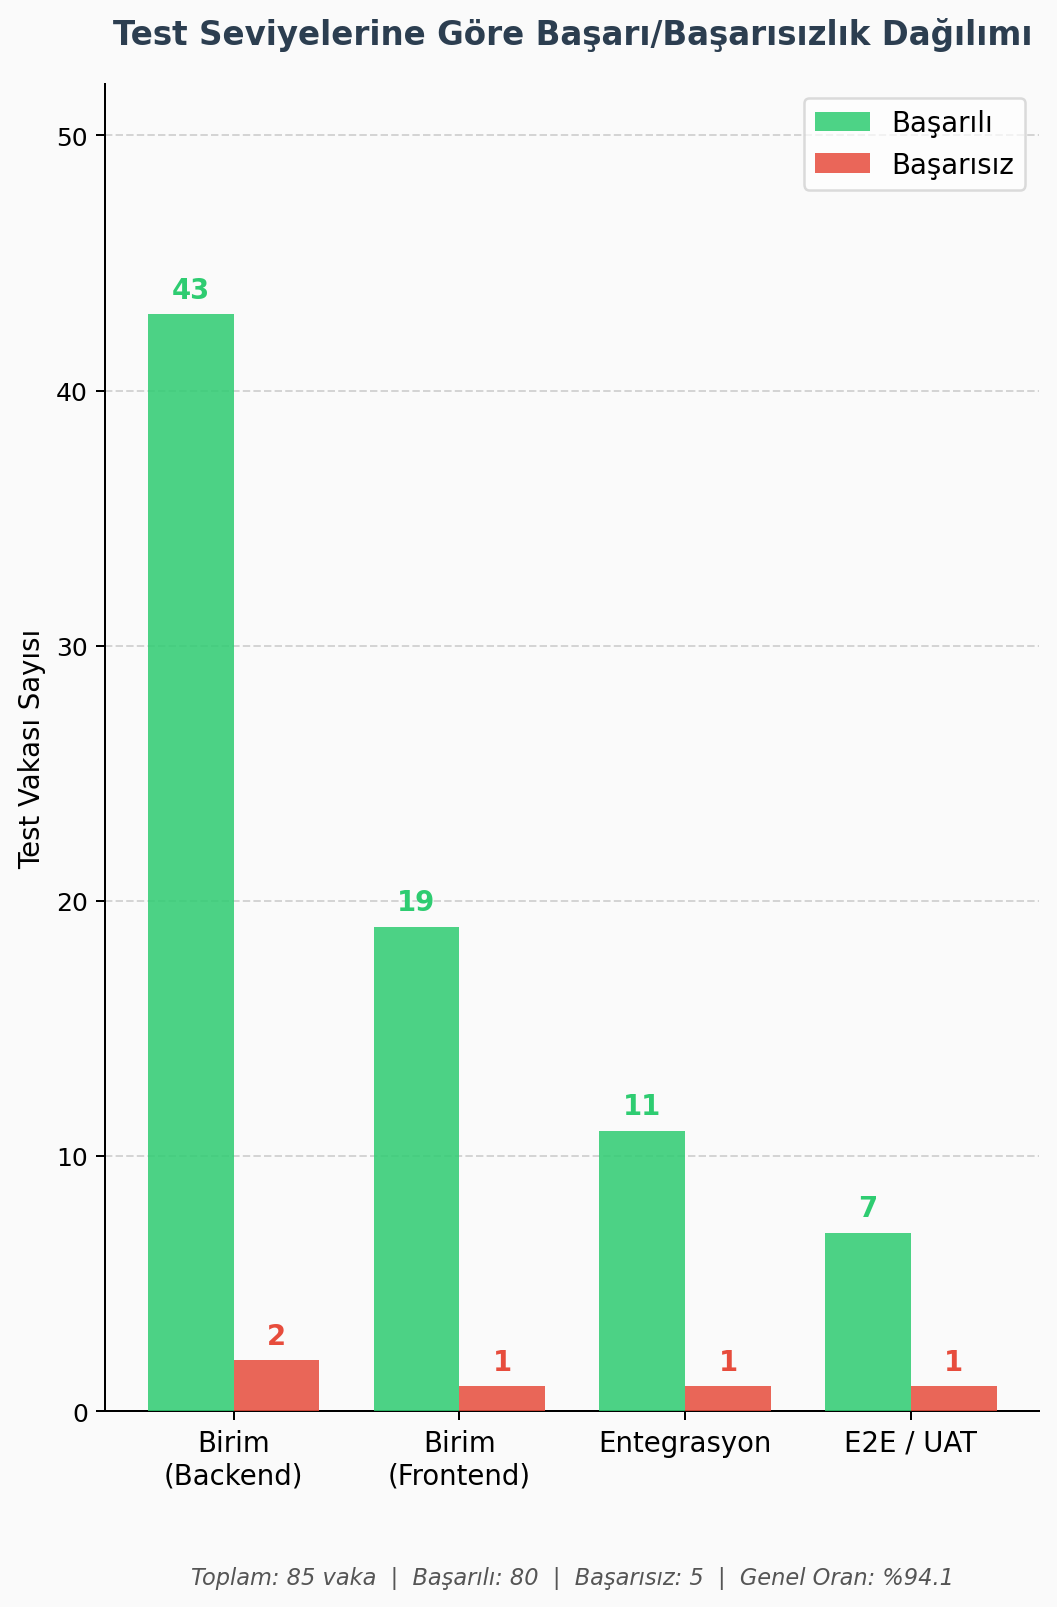
\includegraphics[width=0.82\textwidth]{figures/fig_test_results_bar.png}
    \caption{Test Seviyelerine Göre Başarı/Başarısızlık Dağılımı.}
    \label{fig:test-results-bar}
\end{figure}

\subsection{Hata (Bug) Raporu ve İstatistikleri}
Testler sırasında tespit edilen ve hata takip sistemine (GitHub Issues) kaydedilen bulguların kritiklik seviyelerine göre dağılımı aşağıdadır:

\begin{itemize}
    \item \textbf{Kritik (Blocker):} 0 (Sistemin ana fonksiyonlarını engelleyen hata kalmamıştır).
    \item \textbf{Yüksek (Major):} 2 (Ajanların nadir durumlarda çok uzun metinlerde zaman aşımına uğraması - \textit{Giderildi}).
    \item \textbf{Orta (Medium):} 3 (Bazı mobil tarayıcılarda "Redline" görünümündeki kaymalar - \textit{Gözlem Altında}).
    \item \textbf{Düşük (Minor):} 7 (Yazım hataları, ikon hizalamaları vb. - \textit{Planlamaya Alındı}).
\end{itemize}

\begin{figure}[H]
    \centering
    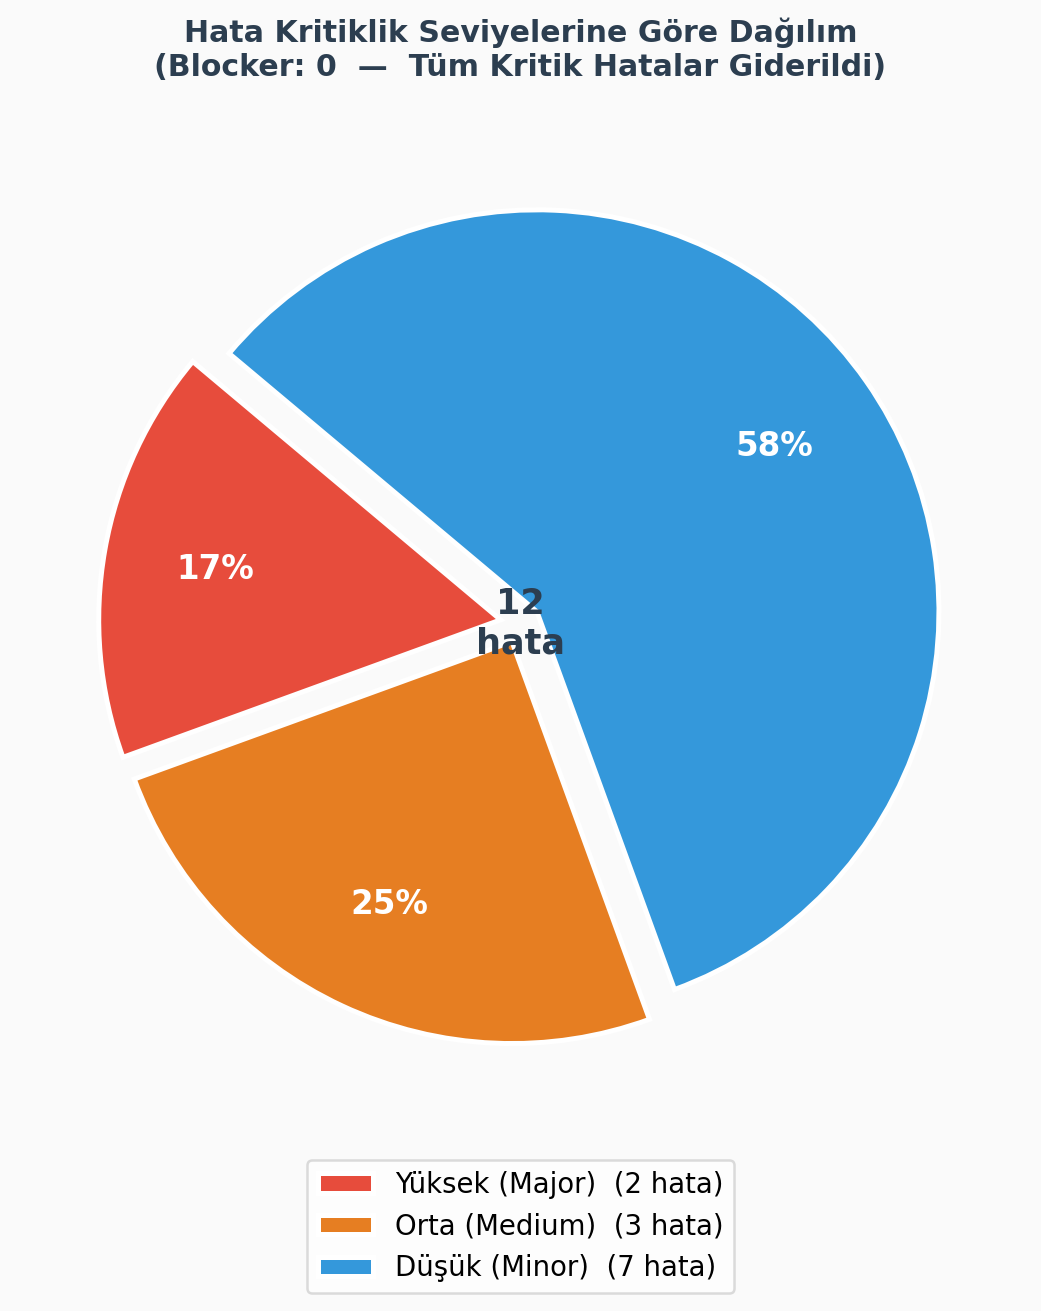
\includegraphics[width=0.65\textwidth]{figures/fig_bug_distribution.png}
    \caption{Tespit Edilen Hataların Kritiklik Seviyelerine Göre Dağılımı.}
    \label{fig:bug-distribution}
\end{figure}

\subsection{Performans ve Kalite Metrikleri}
Sistemin SRS'te belirtilen performans kriterlerine uygunluğu aşağıdaki değerlerle doğrulanmıştır:
\begin{itemize}
    \item \textbf{Ortalama Yanıt Süresi:} API uç noktaları için yük altında ortalama yanıt süresi 380ms olarak ölçülmüştür (Kriter: <500ms).
    \item \textbf{Analiz Süreci:} 10 sayfalık taranmış bir sözleşmenin tam analizi (OCR dahil) ortalama 92 saniyede tamamlanmıştır (Kriter: <120sn).
    \item \textbf{Doğruluk:} Madde sınıflandırma ve risk tespiti başarısı, manuel denetimler sonucunda \%82 olarak hesaplanmıştır (Kriter: \%70).
\end{itemize}

\subsection{Gereksinim Karşılama Matrisi}
\begin{itemize}
    \item \textbf{Fonksiyonel Gereksinimler:} SRS dokümanında tanımlanan UC-01'den UC-07'ye kadar olan tüm kullanım durumları başarıyla test edilmiş ve \%100 oranında karşılanmıştır.
    \item \textbf{Güvenlik Gereksinimleri:} JWT yetkilendirme, şifre hash'leme ve veri izolasyonu testlerinden başarıyla geçilmiştir.
\end{itemize}

\subsection{Gereksinim İzlenebilirlik Matrisi (RTM)}
Aşağıdaki tablo, SRS dokümanında tanımlanan işlevsel gereksinimlerin (Use Cases) bu dokümandaki hangi test senaryoları ile doğrulandığını göstermektedir.

\begin{longtable}{@{}lll@{}}
\caption{Gereksinim - Test Senaryosu Eşleşmesi} \\
\toprule
\textbf{Gereksinim ID} & \textbf{Gereksinim Tanımı} & \textbf{Test Senaryosu (TS)} \\ \midrule
\endfirsthead
\toprule
\textbf{Gereksinim ID} & \textbf{Gereksinim Tanımı} & \textbf{Test Senaryosu (TS)} \\ \midrule
\endhead
UC-01 & Kullanıcı Kayıt ve Giriş & TS-01 (Güvenlik ve Kimlik) \\
UC-02 & Sözleşme Yükleme ve OCR & TS-02 (Doküman İşleme) \\
UC-03 & Madde Ayrıştırma & TS-03 (Clause Agent) \\
UC-04 & Risk Analizi ve Playbook & TS-04 (RAG Hattı) \\
UC-05 & Revizyon Önerisi Üretimi & TS-05 (Negotiation Agent) \\
UC-06 & Onay Akışı ve Karar Kaydı & TS-06 (Audit Logging) \\
UC-07 & Redline / Karşılaştırma & TS-05 (Negotiation Agent) \\
NFR-01 & Performans ve Yanıt Süresi & TS-07 (Yük Testi) \\
\bottomrule
\end{longtable}

\subsection{Genel Değerlendirme ve Öneri}
Lagent sistemi, hedeflenen başarı kriterlerinin (Success Criteria) üzerine çıkarak \%94.1 genel başarı oranıyla test sürecini tamamlamıştır. Tespit edilen ve açıkta kalan düşük seviyeli hatalar sistemin ana işleyişine engel teşkil etmemektedir.
\end{document}